%% icnonla23.tex
%% Copyright 2023 Tom M. Ragonneau
\documentclass[optimization]{common/talk}
\usepackage{makecell}
\usetikzlibrary{patterns}

\title{COBYQA}
\subtitle{A derivative-free trust-region SQP method for nonlinearly constrained optimization}
\date{ICNONLA 2023, Taiyuan, China, 2023}
\author{\href{https://www.tomragonneau.com}{\textbf{Tom M. Ragonneau}} \and \href{https://www.zhangzk.net}{Zaikun Zhang}}
\institute{
    Department of Applied Mathematics\\
    The Hong Kong Polytechnic University\\
    Hung Hom, Kowloon, Hong Kong, China\\[\baselineskip]
    This work was partially supported by the \href{https://cerg1.ugc.edu.hk/hkpfs/index.html}{Hong Kong PhD Fellowship Scheme}.
}
\hypersetup{
    pdfsubject={ICNONLA 2023},
    pdfkeywords={},
}

\begin{document}

\maketitle

\begin{frame}{Derivative-free optimization}
    \begin{itemize}
        \item Minimize a function $\obj$ using \alert{function values} but no derivatives.
        \item $\obj$ can be a \alert{black box} resulting from experiments or simulations.
        \begin{center}
            \medskip
            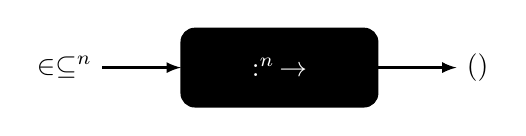
\begin{tikzpicture}
                \draw[-latex,thick] (0,0) node[left] {$\iter \in \fset \subseteq \R^n$} -- (1,0);
                \draw[rounded corners=5pt,fill=black] (1,-.5) rectangle (3.5,.5);
                \node[color=white] at (2.25,0) {$\obj \colon \R^n \to \R$};
                \draw[-latex,thick] (3.5,0) -- (4.5,0) node[right] {$\obj ( \iter )$};
            \end{tikzpicture}
        \end{center}
        \item $\obj$ may be smooth, but $\gradobj$ \alert{cannot} be numerically evaluated.
        \item Evaluations of $\obj$ can be \alert{noisy} and \alert{expensive}.
        \begin{center}
            \medskip
            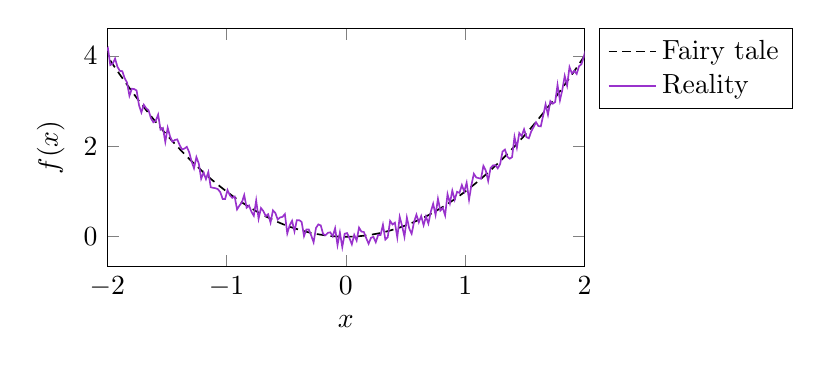
\begin{tikzpicture}
                \begin{axis}[scale only axis=true,width=.5\textwidth,height=.25\textwidth,legend pos=outer north east,legend cell align=left,xmin=-2,xmax=2,xlabel={$x$},ylabel={$f(x)$}]
                    \addplot[no markers,densely dashed,semithick,smooth,samples=50] {x*x};
                    \addplot[no markers,semithick,DarkOrchid,samples=500] {x*x+.25*rand};
                    \legend{Fairy tale,Reality}
                \end{axis}
            \end{tikzpicture}
        \end{center}
    \end{itemize}
\end{frame}

\begin{frame}{An example of a derivative-free optimization problem}
    \begin{center}
        \begin{tikzpicture}[scale=.9, every node/.style={transform shape}]
            \uncover<2>{\draw[pattern=north west lines,pattern color=DarkCaramel!40,rounded corners=5pt] (8,3) rectangle (11,4.5);}
            \draw[thick,rounded corners=5pt] (0,0) rectangle (3,1.5);
            \draw[thick,rounded corners=5pt] (0,4) rectangle (3,5.5);
            \draw[thick,rounded corners=5pt] (4,2) rectangle (7,3.5);
            \draw[thick,rounded corners=5pt] (8,1) rectangle (11,2.5);
            \only<1>{\draw[thick,rounded corners=5pt] (8,3) rectangle (11,4.5);}
            \uncover<2>{\draw[thick,rounded corners=5pt,color=DarkCaramel] (8,3) rectangle (11,4.5);}
            \draw[thick,-latex] (3,1) -- (5.5,1) -- (5.5,2);
            \draw[thick] (3,0.5) -- (7.5,0.5) -- (7.5,2.5) -- (7,2.5);
            \draw[thick,-latex] (7.5,1.75) -- (8,1.75);
            \draw[thick] (3,4.75) -- (7.5,4.75) -- (7.5,3) -- (7,3);
            \draw[thick,-latex] (7.5,3.75) -- (8,3.75);
            \node at (0.6,0.75) {\includegraphics[height=0.75cm]{img/presentation.png}};
            \node at (0.6,4.75) {\includegraphics[height=0.75cm]{img/checklist.png}};
            \node at (4.6,2.75) {\includegraphics[height=0.75cm]{img/deep-learning.png}};
            \node at (8.6,1.75) {\includegraphics[height=0.75cm]{img/good.png}};
            \node at (8.6,3.75) {\includegraphics[height=0.75cm]{img/result.png}};
            \node at (2,0.75) {\makecell{Training\\ data}};
            \node at (2,4.75) {\makecell{Testing\\ data}};
            \node at (6,2.75) {\makecell{Machine\\ learning\\ model}};
            \node at (10,1.75) {\makecell{Training\\ accuracy}};
            \node at (10,3.75) {\makecell{Testing\\ accuracy}};
            \uncover<2>{
                \draw[pattern=north west lines,pattern color=DarkCaramel!40,rounded corners=5pt] (0,2) rectangle (3,3.5);
                \draw[thick,color=DarkCaramel,rounded corners=5pt] (0,2) rectangle (3,3.5);
                \draw[thick,-latex] (3,2.75) -- (4,2.75);
                \node at (0.6,2.75) {\includegraphics[height=0.75cm]{img/technical-support.png}};
                \node at (2,2.75) {\makecell{Hyper-\\parameters}};
            }
        \end{tikzpicture}

        \pause
        \medskip

        \begin{block}{Hyperparameter tuning problem}
            How to choose the \alert{hyperparameters} of a machine learning model?
        \end{block}
    \end{center}
\end{frame}

\begin{frame}{General context}
    We design a method named \alert{COBYQA} for solving
    \begin{equation*}
        \begin{aligned}
            \min_{\iter \in \R^n}   & \quad \obj ( \iter ) \\
            \textrm{s.t.}           & \quad \cub ( \iter ) \le 0, ~ \cancel<2->{\ceq ( \iter ) = 0},\\
                                    & \quad \xl \le \iter \le \xu,
        \end{aligned}
    \end{equation*}
    when derivatives of $\obj$, $\cub$, and $\ceq$ are \alert{unavailable}.

    \pause
    \medskip

    \begin{block}{}
        \begin{itemize}[<+->]
            \item We omit the equality constraints for simplicity.
            \item COBYQA aims at being a \alert{successor} to COBYLA \cite{Powell_1994}.
            \item We \alert{implement} COBYQA into a Python solver.
            \item The bound constraints are \alert{unrelaxable}:
            \begin{itemize}
                \item They often represent \alert{inalienable} restrictions.
                \item $\obj$ or $\cub$ may not be defined outside of the bounds.
            \end{itemize}
        \end{itemize}
    \end{block}
\end{frame}

\begin{frame}{Table of contents}
    \tableofcontents[hideallsubsections]
\end{frame}

\section{General framework of COBYQA}

\begin{frame}{A derivative-free trust-region SQP method}
    To do.
\end{frame}

\begin{frame}[allowframebreaks]{References}
    \bibliography{\bibfile}
\end{frame}

\end{document}
